\documentclass[a4paper,12pt]{article}

% Paquetes básicos
\usepackage[utf8]{inputenc}
\usepackage[T1]{fontenc}
\usepackage[spanish]{babel}
\usepackage{graphicx}
\usepackage{xcolor}
\usepackage{lipsum}
\usepackage{geometry}
\geometry{top=3cm, bottom=3cm, left=2.5cm, right=2.5cm}

% Paquetes para diseño
\usepackage{titlesec}
\usepackage{fancyhdr}
\usepackage{amsmath}
\usepackage{textgreek}
\usepackage{amssymb}
\usepackage{hyperref}

% Paquetes para el entorno lstlisting
\usepackage{listings}
\usepackage{inconsolata}

%encabezado y pie de página nivel profesional
\usepackage{fancyhdr}
\pagestyle{fancy}
\fancyhf{}
\fancyhead[L]{\leftmark}
\fancyhead[R]{\rightmark}
\fancyfoot[L]{\textbf{Ismael Sallami Moreno - GIIADE}}
\fancyfoot[C]{\thepage}
\fancyfoot[R]{\textbf{(UGR)} \today}
\renewcommand{\headrulewidth}{0.4pt}
\renewcommand{\footrulewidth}{0.4pt}
\setlength{\headheight}{15pt}
\setlength{\headsep}{10pt}
\setlength{\footskip}{20pt}
\usepackage{truncate}
\fancyhead[L]{\truncate{0.5\headwidth}{\leftmark}}
\fancyhead[R]{\truncate{0.5\headwidth}{\rightmark}}
\usepackage{mathpazo}
\usepackage{tcolorbox}
\usepackage{array}



% Paquete para fondo
\usepackage{background}
\usepackage{float}

% Configuración de lstlisting
\lstset{
    inputencoding=utf8,          % Permite UTF-8
    extendedchars=true,          % Reconoce caracteres extendidos
    literate=                    % Configuración manual para tildes y símbolos
        {á}{{\'a}}1
        {é}{{\'e}}1
        {í}{{\'i}}1
        {ó}{{\'o}}1
        {ú}{{\'u}}1
        {ñ}{{\~n}}1
        {Á}{{\'A}}1
        {É}{{\'E}}1
        {Í}{{\'I}}1
        {Ó}{{\'O}}1
        {Ú}{{\'U}}1
        {Ñ}{{\~N}}1
        {¿}{{\textquestiondown}}1
        {¡}{{\textexclamdown}}1,
    basicstyle=\ttfamily,        % Fuente monoespaciada
    breaklines=true,             % Habilita salto de línea automático
    frame=single,                % Marco alrededor del código
    backgroundcolor=\color{gray!10}, % Fondo gris claro
    keywordstyle=\color{blue},   % Color para palabras clave
    commentstyle=\color{green},  % Color para comentarios
    stringstyle=\color{red}      % Color para strings
}
\lstdefinestyle{customcpp}{
    language=C++,                % Lenguaje de programación
    showspaces=false,            % No mostrar espacios
    showtabs=false,              % No mostrar tabulaciones
    tabsize=4,                   % Tamaño de tabulación
    showstringspaces=false,      % No mostrar espacios en strings
    numbers=left,                % Números de línea a la izquierda
    numberstyle=\tiny\color{gray}, % Estilo de los números de línea
    numbersep=5pt,               % Separación de los números de línea
    stepnumber=1,                % Mostrar número en cada línea
    basicstyle=\ttfamily\footnotesize, % Estilo básico del código
    keywordstyle=\bfseries\color{blue}, % Estilo de las palabras clave
    commentstyle=\itshape\color{green!50!black}, % Estilo de los comentarios
    stringstyle=\color{red},     % Estilo de los strings
    identifierstyle=\color{black}, % Estilo de los identificadores
    % procnamekeys={def,class},    % Palabras clave para nombres de funciones
    morekeywords={constexpr,nullptr,size_t}, % Más palabras clave
    emph={int,char,double,float,unsigned}, % Palabras a enfatizar
    emphstyle=\color{magenta},   % Estilo de las palabras enfatizadas
    backgroundcolor=\color{gray!10}, % Color de fondo
    frame=shadowbox,             % Marco con sombra
    rulesepcolor=\color{gray},   % Color de la línea de separación
    breakatwhitespace=false,     % No cortar en espacios en blanco
    breaklines=true,             % Cortar líneas largas
    captionpos=b,                % Posición del título (abajo)
    escapeinside={(*@}{@*)},     % Delimitadores para escapar a LaTeX
    morecomment=[l][\color{magenta}]{\#}, % Comentarios de una línea
    morecomment=[s][\color{orange}]{/*}{*/}, % Comentarios multilínea
    morestring=[b],             % Strings entre comillas dobles
    morestring=[b]'              % Strings entre comillas simples
}

% Configuración de título
\titleformat{\section}{\normalfont\Large\bfseries}{\thesection}{1em}{}

% Información del documento
\title{
    \vspace{-2cm}
    
\includegraphics[width=0.3\textwidth]{images/etsiit.png} \\ % Cambia el logo si es necesario
    \LARGE Ingeniería Informática + ADE\\
    \large Universidad de Granada (UGR)\\[1cm]
}
\author{\textbf{Autor:} Ismael Sallami Moreno}
\date{\textbf{Asignatura:} Tema 4: Seguridad en Redes (FR)\\[1cm]}

% Configuración del fondo
\backgroundsetup{
    scale=1,
    color=black,
    opacity=0.2,
    angle=0,
    position=current page.south,
    vshift=0pt,
    hshift=0pt,
    contents={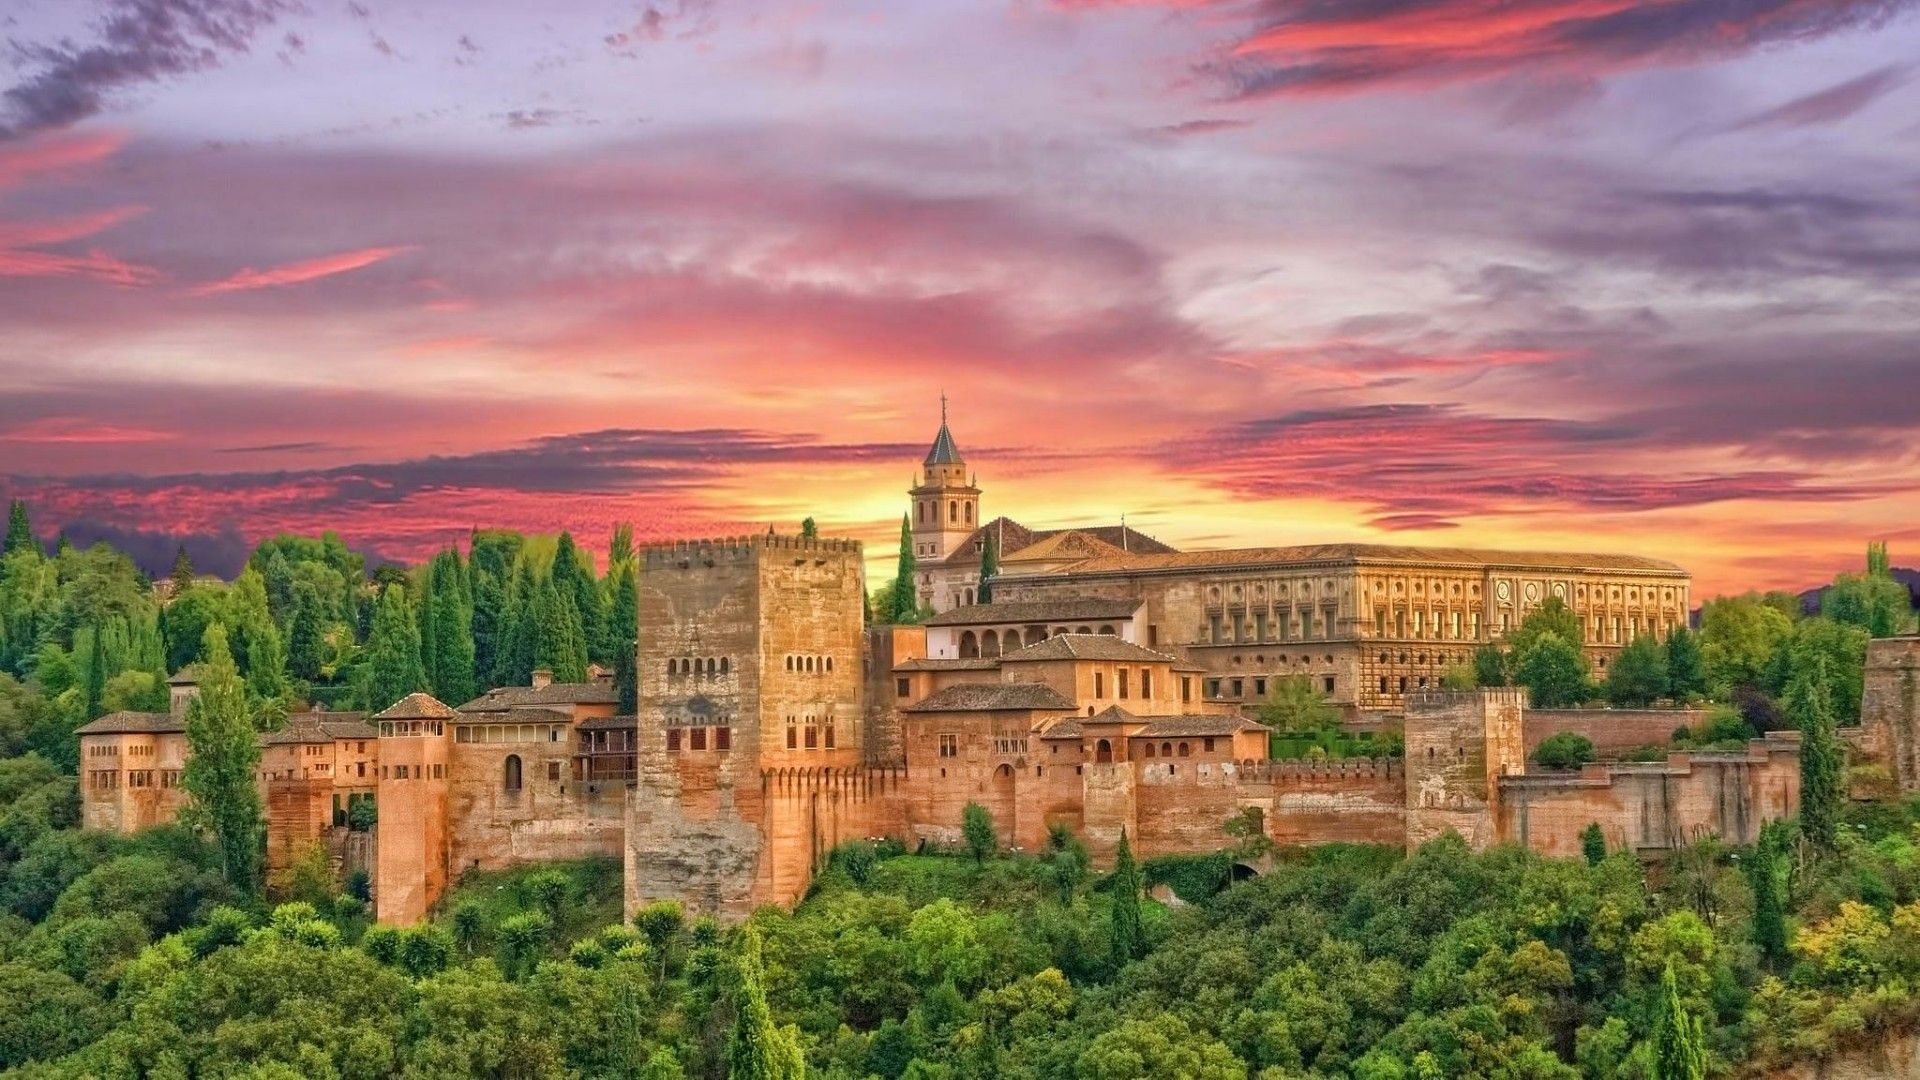
\includegraphics[width=\paperwidth,height=\paperheight,keepaspectratio]{images/granada.jpg}}
}

% Inicio del documento
\begin{document}

% Portada
\maketitle
\thispagestyle{empty}

\begin{center}
    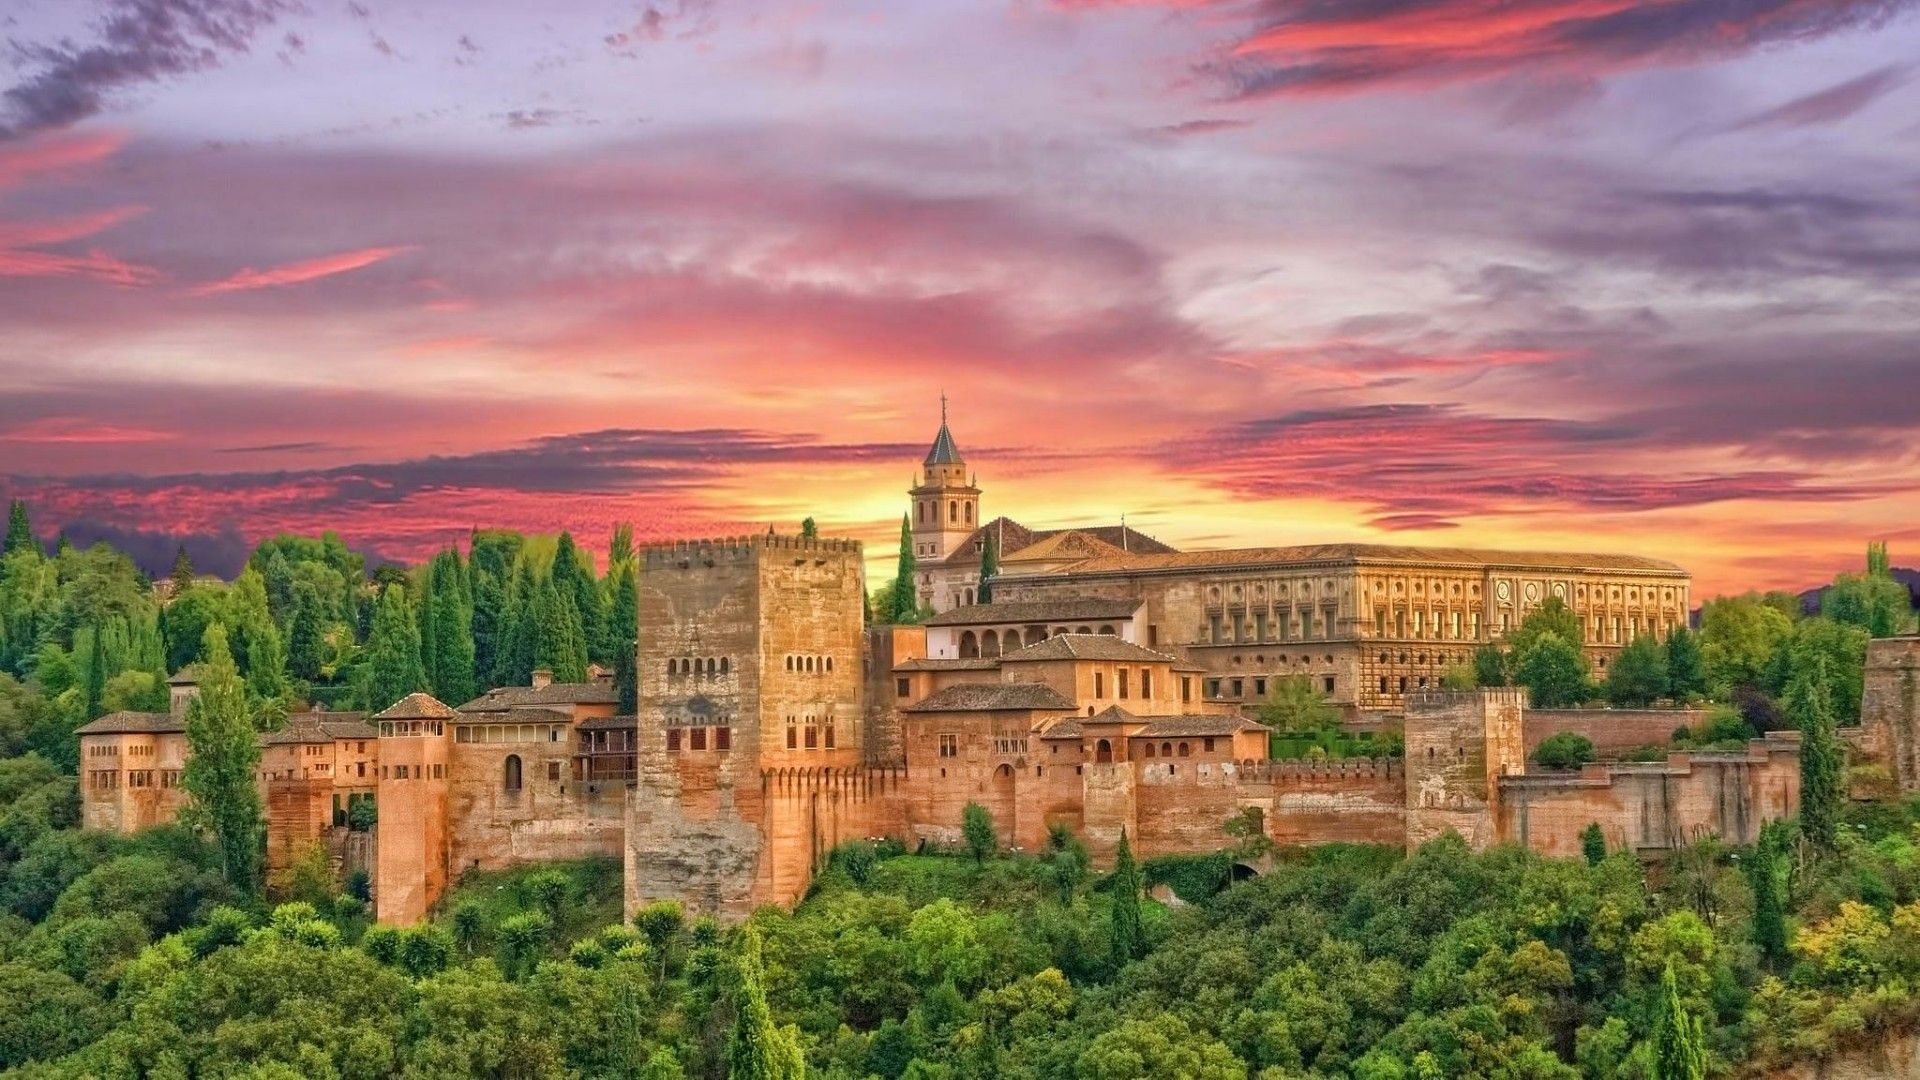
\includegraphics[width=\textwidth,height=0.4\textheight,keepaspectratio]{images/granada.jpg} \\ % Añade tu imagen de fondo
    \vfill
\end{center}

\newpage

% Índice (opcional)
\tableofcontents
\newpage


\section{Introducción}

Una red de comunicaciones se considera \textbf{segura} cuando se garantiza la protección de todos los aspectos clave de la seguridad. Sin embargo, es importante destacar que \textbf{no existen protocolos ni redes 100\% seguras}.

\subsection{¿Qué es la seguridad?}

La seguridad en redes engloba múltiples aspectos fundamentales:

\begin{itemize}
    \item \textbf{Confidencialidad/Privacidad:} El contenido de la información debe ser comprensible únicamente para las entidades autorizadas.
    \item \textbf{Autenticación:} Garantiza que las entidades involucradas son quienes afirman ser.
    \item \textbf{Control de accesos:} Los servicios deben estar accesibles solo a entidades autorizadas.
    \item \textbf{No repudio o irrenunciabilidad:} Impide que una entidad niegue haber realizado una acción determinada.
    \item \textbf{Integridad:} El sistema debe detectar cualquier alteración de la información, ya sea intencionada o accidental.
    \item \textbf{Disponibilidad:} Los servicios deben mantenerse operativos, independientemente de la demanda.
\end{itemize}

\subsection{¿En qué nivel o capa se debe situar la seguridad?}

La seguridad debe aplicarse en \textbf{todas las capas del sistema}. El grado de seguridad siempre estará limitado por el punto más débil de la red.

\subsection{Mecanismos de Seguridad}

Para garantizar los aspectos mencionados, se utilizan los siguientes mecanismos:

\begin{itemize}
    \item \textbf{Cifrado:} Puede ser simétrico o asimétrico.
    \item \textbf{Autenticación con clave secreta:} Utilizando mecanismos de reto-respuesta.
    \item \textbf{Intercambio de Diffie-Hellman:} Permite establecer claves secretas de forma segura.
    \item \textbf{Funciones Hash:} Como el código de autenticación de mensajes (\textit{Hash Message Authentication Code, HMAC}).
    \item \textbf{Firma Digital:} Para garantizar la autenticidad e integridad de los mensajes.
    \item \textbf{Certificados Digitales:} Utilizados para validar identidades.
\end{itemize}

\subsection{Ataques de Seguridad}

Un \textbf{ataque de seguridad} se define como cualquier acción, intencionada o no, que compromete alguno de los aspectos de la seguridad. Entre los ataques más comunes se encuentran:

\begin{itemize}
    \item \textbf{Sniffing:} También conocido como ''escuchas'' o \textit{husmeo}, vulnera la confidencialidad al interceptar información.
    \item \textbf{Spoofing (phishing):} Suplantación de identidad de entidades legítimas.
    \item \textbf{Man in the Middle:} Ataques de interceptación donde un tercero se posiciona entre las entidades comunicantes.
    \item \textbf{Denegación de Servicio Distribuida (DDoS):} Ejemplo de este ataque es el \textit{flooding} o inundación de solicitudes para colapsar un sistema.
    \item \textbf{Malware:} Incluye amenazas como troyanos, gusanos, \textit{spyware}, puertas traseras (\textit{backdoors}), \textit{rootkits}, ransomware y \textit{keyloggers}.
\end{itemize}



\section{Cifrado}

\textbf{Cifrado de datos:}

\begin{itemize}
    \item Es un procedimiento diseñado para garantizar la \textbf{confidencialidad} de la información.
    \item Consiste en transformar un \textbf{texto llano o claro} (\(P\)) en un \textbf{texto cifrado} (\(C\)).
    \item Este proceso se basa en la utilización de un algoritmo de \textbf{cifrado/descifrado}, comúnmente representado como \(E_K()\) para cifrado y \(D_{K'}()\) para descifrado.
    \item La complejidad del proceso radica en la utilización de una \textbf{clave de cifrado} (\(K\)) y una \textbf{clave de descifrado} (\(K'\)), las cuales deben permanecer desconocidas para garantizar la seguridad del sistema.
\end{itemize}

\begin{figure}[H]
    \centering
    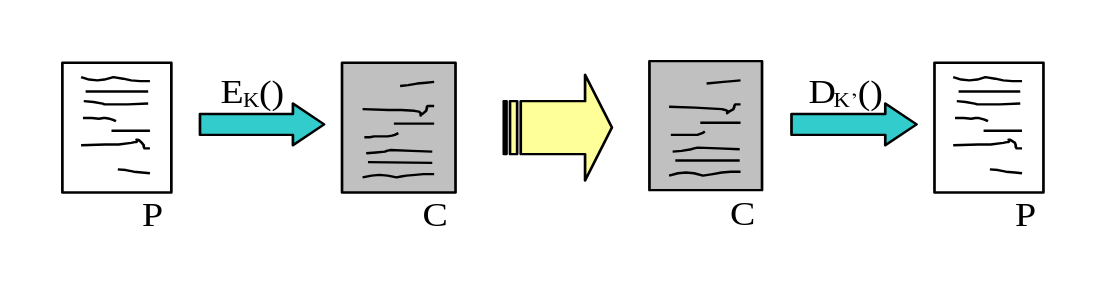
\includegraphics[width=0.8\textwidth]{images/cifrado.png}
    \caption{Esquema de cifrado de datos.}
\end{figure}
\newpage
\subsection{Cifrado simétrico}
\textbf{Cifrado simétrico: Algoritmos de clave secreta}

\begin{itemize}
    \item Utiliza una \textbf{única clave} para realizar tanto el cifrado como el descifrado, es decir, \(K = K'\).
    \item Un ejemplo representativo es el \textbf{DES} (\textit{Data Encryption Standard}), desarrollado por IBM en 1975.
\end{itemize}

\textbf{Enlaces relacionados:}
\begin{itemize}
    \item \href{http://en.wikipedia.org/wiki/Feistel_network}{Estructura Feistel}\footnote{Puedes pinchar en los nombres para acceder a los enlaces}: Explicación de la arquitectura utilizada en muchos algoritmos de cifrado, incluido DES.
    \item \href{http://en.wikipedia.org/wiki/Data_Encryption_Standard}{Data Encryption Standard}: Detalles técnicos y evolución histórica del algoritmo.
\end{itemize}


\begin{figure}[H]
    \centering
    \begin{minipage}{0.45\textwidth}
        \centering
        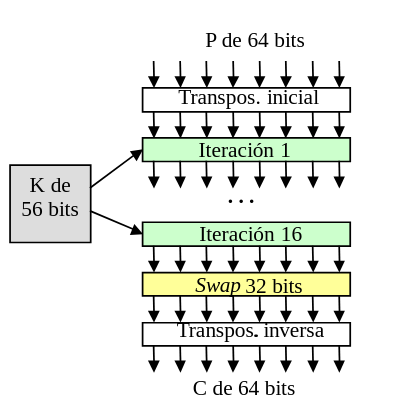
\includegraphics[width=\textwidth]{images/crifrado_a.png}
        \caption{Diagrama A}
    \end{minipage}
    \hfill
    \begin{minipage}{0.45\textwidth}
        \centering
        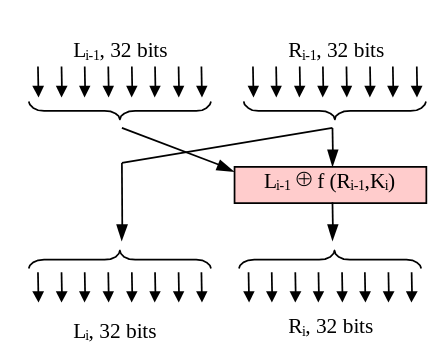
\includegraphics[width=\textwidth]{images/cifrado_b.png}
        \caption{Diagrama B}
    \end{minipage}
\end{figure}

\begin{itemize}
    \item Diagrama A:
    \begin{itemize}
        \item \textbf{P de 64 bits} (plaintext) pasa por una \textbf{Transpos. inicial} (permutación inicial).
        \item El resultado se somete a 16 iteraciones (\textbf{Iteración 1} a \textbf{Iteración 16}) utilizando una \textbf{K de 56 bits} (clave de 56 bits).
        \item Después de las iteraciones, ocurre un \textbf{Swap 32 bits}.
        \item Finalmente, se aplica la \textbf{Transpos. inversa} (permutación inversa) para producir el \textbf{C de 64 bits} (ciphertext).
    \end{itemize}
    \item Diagrama B:
    \begin{itemize}
        \item El \textbf{entrada de 64 bits} se divide en dos mitades de 32 bits, \textbf{Li-1, 32 bits} y \textbf{Ri-1, 32 bits}.
        \item \textbf{Li-1} se combina con el resultado de una función \textbf{f} aplicada a \textbf{Ri-1} y una subclave \textbf{Ki} usando la operación XOR (\(\oplus\)).
        \item La salida es dos mitades de 32 bits, \textbf{Li, 32 bits} y \textbf{Ri, 32 bits}.
    \end{itemize}        
\end{itemize}

\begin{itemize}
    \item \textbf{DES:} Es un esquema de \textbf{sustitución monoalfabética}, lo que significa que cada símbolo del texto plano se sustituye por otro, según un esquema fijo basado en la clave.
    \item \textbf{Encadenamiento DES:} Introducido para evitar que DES actúe como un simple algoritmo de sustitución. Este mecanismo encadena los bloques cifrados, asegurando que cada bloque de texto cifrado dependa no solo del bloque actual de texto claro, sino también del bloque anterior de texto cifrado. Esto incrementa significativamente la seguridad del algoritmo.
    \item Para mejorar la robustez del cifrado, se utilizan variantes como \textbf{2DES} y \textbf{3DES}. 
    \begin{itemize}
        \item \textbf{2DES (Double DES):} Consiste en aplicar el algoritmo DES dos veces consecutivas con dos claves diferentes. Aunque incrementa la seguridad en comparación con DES simple, sigue siendo vulnerable a ciertos tipos de ataques, como el ataque de encuentro en el medio (\textit{meet-in-the-middle}).
        \item \textbf{3DES (Triple DES):} Aplica el algoritmo DES tres veces, generalmente con dos o tres claves diferentes. Este método es mucho más seguro que DES y 2DES, y ha sido ampliamente utilizado en la industria para proteger datos sensibles.
    \end{itemize}
\end{itemize}

\begin{figure}[H]
    \centering
    \begin{minipage}{0.45\textwidth}
        \centering
        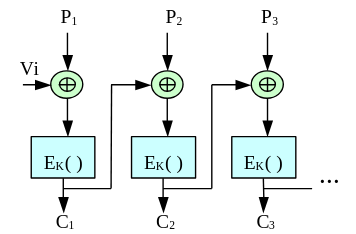
\includegraphics[width=\textwidth]{images/des_A.png}
        \caption{Diagrama A}
    \end{minipage}
    \hfill
    \begin{minipage}{0.45\textwidth}
        \centering
        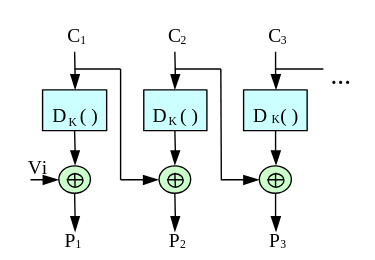
\includegraphics[width=\textwidth]{images/des_B.png}
        \caption{Diagrama B}
    \end{minipage}
    \hfill
    \begin{minipage}{0.6\textwidth}
        \centering
        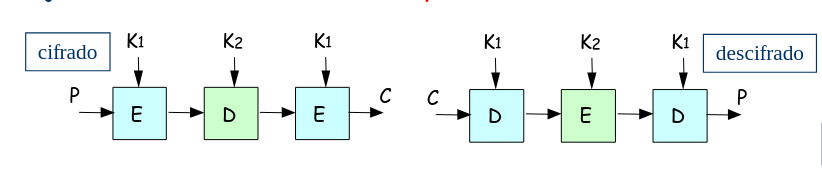
\includegraphics[width=\textwidth]{images/des2_y_3des.png}
        \caption{Diagrama 2 y 3DES}
    \end{minipage}
\end{figure}


\newpage

\textbf{IDEA (\textit{International Data Encryption Algorithm, IDEA})}

\begin{itemize}
    \item Es un algoritmo de cifrado \textbf{simétrico}, lo que significa que utiliza la \textbf{misma clave} tanto para cifrar como para descifrar.
    \item Utiliza \textbf{claves de 128 bits}, proporcionando un alto nivel de seguridad.
    \item Diseñado para \textbf{operar en tiempo real}, con implementación eficiente en hardware (\textit{Very Large Scale Integration, VLSI}).
\end{itemize}

\begin{figure}[H]
    \centering
    \begin{minipage}{0.45\textwidth}
        \centering
        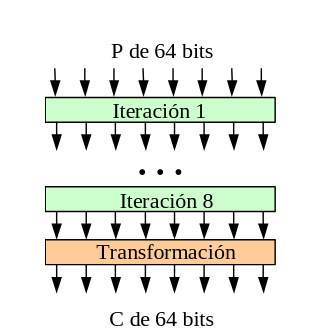
\includegraphics[width=\textwidth]{images/ideaA.png}
        \caption{Diagrama A}
    \end{minipage}
    \hfill
    \begin{minipage}{0.45\textwidth}
        \centering
        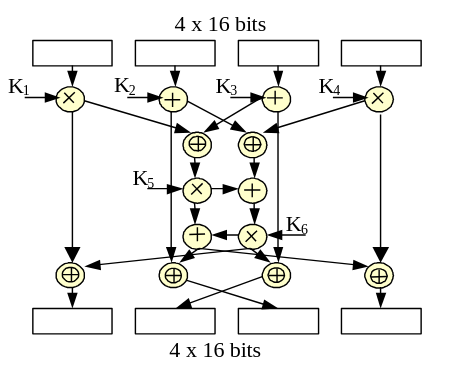
\includegraphics[width=\textwidth]{images/ideaB.png}
        \caption{Diagrama B}
    \end{minipage}
\end{figure}

\subsection{Cifrado asimétrico}

\textbf{Cifrado asimétrico: Algoritmos de clave pública/privada}

\begin{itemize}
    \item Cada usuario (\(A\)) posee dos claves distintas:
    \begin{itemize}
        \item Una \textbf{clave pública} (\(K_{\text{PUB}_A}\)).
        \item Una \textbf{clave privada} (\(K_{\text{PRI}_A}\)).
    \end{itemize}
    \item Conociendo \(K_{\text{PUB}_A}\), es \textbf{imposible deducir} \(K_{\text{PRI}_A}\).
    \item Las claves son diferentes para las operaciones de cifrado y descifrado:
    \begin{itemize}
        \item \textbf{Cifrado:} \(C = E_{K_{\text{PUB}_B}}(P)\), donde \(P\) es el texto plano.
        \item \textbf{Descifrado:} \(P = D_{K_{\text{PRI}_B}}(C)\), donde \(C\) es el texto cifrado.
    \end{itemize}
    \item En caso de enviar \(C = E_{K_{\text{PRI}_A}}(P)\), el receptor puede verificar la \textbf{autenticidad} del mensaje al descifrarlo con \(K_{\text{PUB}_A}\).
\end{itemize}

\begin{figure}[H]
    \centering
    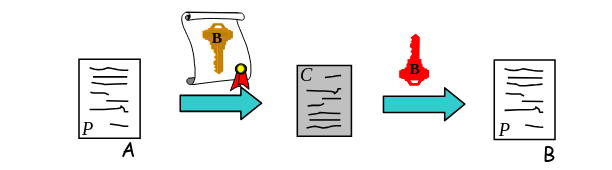
\includegraphics[width=0.8\textwidth]{images/cifrado_asimetrico.png}
    \caption{Esquema de cifrado asimétrico.}
\end{figure}

\textbf{RSA (\textit{Rivest, Shamir y Adleman})}

\begin{itemize}
    \item Se eligen dos números primos grandes \(p\) y \(q\), donde \(p, q > 10^{100}\).
    \item Calculamos:
    \begin{itemize}
        \item \(n = p \cdot q\).
        \item \(z = (p-1) \cdot (q-1)\), utilizando la función de Euler.
    \end{itemize}
    \item Elegimos un número \(d\), primo respecto de \(z\).
    \item Calculamos \(e\) tal que \(e \cdot d \mod z = 1\), utilizando el algoritmo de Euclides.
    \item Las claves generadas son:
    \begin{itemize}
        \item Clave pública: \(K_{\text{PUB}} = (e, n)\).
        \item Clave privada: \(K_{\text{PRI}} = (d, n)\).
    \end{itemize}
    \item Las operaciones de cifrado y descifrado son:
    \begin{itemize}
        \item \textbf{Cifrado:} \(C = P^e \mod n\).
        \item \textbf{Descifrado:} \(P = C^d \mod n\).
    \end{itemize}
\end{itemize}

\textbf{Ejemplo RSA}

\begin{itemize}
    \item Se eligen los valores:
    \begin{itemize}
        \item \(p = 3\), \(q = 11\).
        \item \(n = p \cdot q = 33\).
        \item \(z = (p-1)(q-1) = (3-1)(11-1) = 2 \cdot 10 = 20\).
    \end{itemize}
    \item Elegimos \(d = 7\), un número primo respecto de \(z\).
    \item Calculamos \(e\) tal que \(e \cdot d \mod z = 1\). En este caso, \(e = 3\).
    \item Las claves generadas son:
    \begin{itemize}
        \item Clave pública: \(K_{\text{PUB}} = (3, 33)\).
        \item Clave privada: \(K_{\text{PRI}} = (7, 33)\).
    \end{itemize}
\end{itemize}

\textbf{Cifrado y descifrado}

La siguiente tabla muestra el proceso de cifrado y descifrado para varios caracteres. Utilizamos la notación:

\begin{itemize}
    \item \textbf{Cifrado:} \(C = P^e \mod n\).
    \item \textbf{Descifrado:} \(P = C^d \mod n\).
\end{itemize}

\begin{figure}[H]
    \centering
    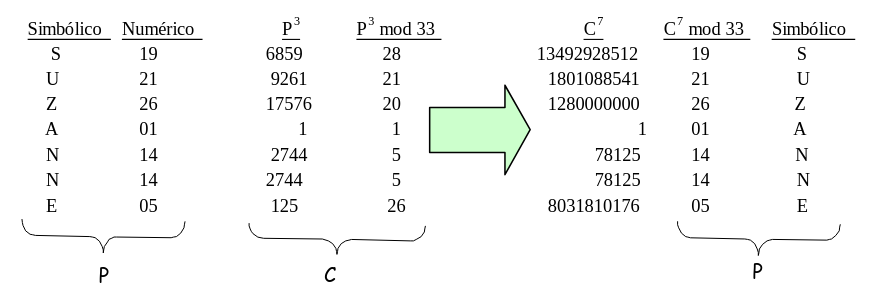
\includegraphics[width=0.8\textwidth]{images/rsa.png}
    \caption{Ejercicio Resuelto RSA.}
\end{figure}

\textbf{Resultado:} El texto original se recupera perfectamente después del cifrado y descifrado, demostrando la efectividad del esquema RSA.

\section{Autenticación}
\subsection{Reto-respuesta}

\begin{itemize}
    \item \textbf{Esquema de reto-respuesta:}
    \begin{itemize}
        \item Este método se utiliza para verificar la identidad de una entidad (por ejemplo, un cliente o servidor) sin necesidad de compartir directamente la clave secreta.
        \item El procedimiento típico es:
        \begin{enumerate}
            \item La entidad que autentica (por ejemplo, el servidor) envía un \textbf{reto} (\(R\)) a la otra entidad (por ejemplo, el cliente).
            \item El cliente responde cifrando el reto con la clave secreta compartida (\(K\)), generando la respuesta cifrada \(C = E_K(R)\).
            \item El servidor descifra la respuesta con la clave compartida y verifica si coincide con el reto original.
        \end{enumerate}
    \end{itemize}
    \item \textbf{¿Ataque por reflexión?}
    \begin{itemize}
        \item Un ataque por reflexión ocurre cuando un atacante intercepta un reto enviado por una entidad y lo devuelve como respuesta, intentando hacerse pasar por una entidad legítima.
        \item Para mitigar este ataque, es importante implementar:
        \begin{itemize}
            \item \textbf{Espacios de claves disjuntos:} Utilizar claves diferentes para cada dirección de comunicación. Por ejemplo:
            \begin{itemize}
                \item \(K_{A \to B}\): Clave utilizada para mensajes enviados de \(A\) a \(B\).
                \item \(K_{B \to A}\): Clave utilizada para mensajes enviados de \(B\) a \(A\).
            \end{itemize}
            \item Esto garantiza que un reto enviado por \(A\) no pueda ser simplemente reflejado de vuelta a \(A\) por \(B\), ya que \(A\) esperará que el mensaje esté cifrado con \(K_{B \to A}\).
        \end{itemize}
    \end{itemize}
\end{itemize}

\textbf{Resumen:} El esquema de reto-respuesta ofrece una manera eficiente de autenticar entidades sin revelar claves secretas. Sin embargo, es crucial implementar contramedidas como los \textbf{espacios de claves disjuntos} para evitar ataques por reflexión.

\begin{figure}[H]
    \centering
    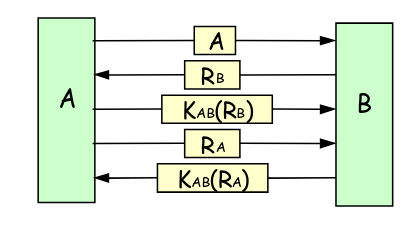
\includegraphics[width=0.8\textwidth]{images/reto_respuesta.png}
    \caption{Esquema de reto-respuesta.}
\end{figure}

\subsection{Intercambio de Diffie-Hellman}

El \textit{intercambio de claves de Diffie-Hellman} es un protocolo de criptografía que permite a dos entidades, A y B, establecer una clave secreta compartida, sin necesidad de intercambiar dicha clave explícitamente. En su lugar, utilizan números públicos y realizan cálculos sobre ellos. A continuación se describen los pasos básicos del protocolo:

\begin{enumerate}
    \item Ambas partes acuerdan un número primo grande \( p \) y una base \( g \), los cuales son públicos.
    \item La parte A elige un número secreto \( a \) y calcula \( A = g^a \mod p \), luego envía \( A \) a la parte B.
    \item La parte B elige un número secreto \( b \) y calcula \( B = g^b \mod p \), luego envía \( B \) a la parte A.
    \item Ambas partes calculan la clave compartida:
    \begin{itemize}
        \item La parte A calcula \( K = B^a \mod p \).
        \item La parte B calcula \( K = A^b \mod p \).
    \end{itemize}
    Como \( A^b \mod p = B^a \mod p \), ambas partes obtienen la misma clave secreta \( K \), que pueden usar para cifrar la comunicación.
\end{enumerate}

Este protocolo es seguro debido a la dificultad del problema de calcular los logaritmos discretos, es decir, dado \( g^a \mod p \) y \( g^b \mod p \), es extremadamente difícil calcular \( a \) o \( b \).

\begin{figure}[H]
    \centering
    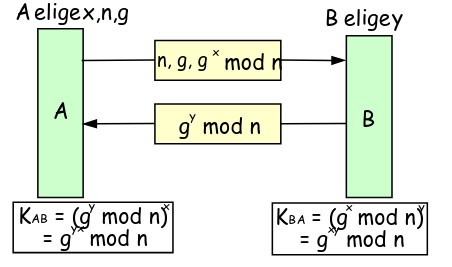
\includegraphics[width=0.8\textwidth]{images/diffie_hellman.png}
    \caption{Intercambio de claves de Diffie-Hellman.}
\end{figure}


\subsubsection{Ataque Man-in-the-Middle (MitM)}

Aunque el intercambio de Diffie-Hellman es seguro, puede ser vulnerable a un \textit{ataque Man-in-the-Middle} (MitM). En este tipo de ataque, un atacante (C) se coloca entre las dos partes A y B, interceptando y alterando los mensajes entre ellas.

\begin{enumerate}
    \item La parte A envía su valor \( A = g^a \mod p \) al atacante (C) en lugar de enviarlo directamente a B.
    \item El atacante (C) elige su propio valor secreto \( c \), calcula \( C = g^c \mod p \) y envía \( C \) a la parte B.
    \item La parte B, al recibir \( C \), calcula la clave \( K_B = C^b \mod p \) y la envía de vuelta al atacante.
    \item El atacante calcula la clave \( K_A = A^c \mod p \), y ahora tiene dos claves secretas: \( K_A \) y \( K_B \).
    \item De esta manera, el atacante puede leer y modificar la comunicación entre A y B sin que ninguna de las partes se dé cuenta.
\end{enumerate}

Este ataque funciona porque A y B creen que están intercambiando información directamente entre sí, pero en realidad están enviando la información al atacante, quien actúa como intermediario.

Para mitigar este tipo de ataque, se pueden usar firmas digitales o certificados, lo que permite a A y B asegurarse de que están comunicándose con la parte correcta.

\begin{figure}[H]
    \centering
    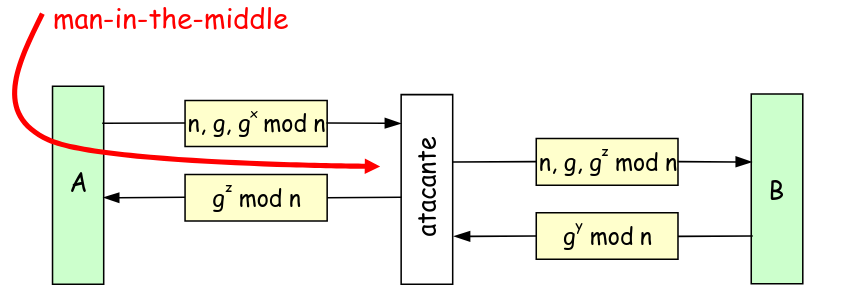
\includegraphics[width=0.8\textwidth]{images/ataque.png}
    \caption{Ataque}
\end{figure}

\section{Funciones Hash}

\subsection{Funciones Hash (Compendios)}

Las funciones hash son algoritmos matemáticos que transforman un mensaje de longitud variable en una secuencia de longitud fija. Son ampliamente utilizadas en criptografía para garantizar la integridad de los datos y otros aspectos de seguridad.

\subsubsection{Características de los Compendios}

Las funciones hash tienen las siguientes características:

\begin{itemize}
    \item \textbf{Funciones unidireccionales (irreversibles):} El cálculo de un hash es sencillo, pero es prácticamente imposible obtener el mensaje original a partir de su resumen hash.
    \item \textbf{Texto de entrada (M) de longitud variable:} El tamaño del mensaje de entrada puede variar, pero siempre se transforma en un resumen de longitud fija.
    \item \( M \rightarrow H(M) \): El mensaje \( M \) se convierte en un hash \( H(M) \), que tiene una longitud fija (por ejemplo, 256 o 512 bits).
    \item \textbf{Imposibilidad de obtener \( M \) a partir de \( H(M) \):} Dado un hash \( H(M) \), es prácticamente imposible encontrar el mensaje \( M \) original.
    \item \textbf{Invulnerabilidad a ataques de colisión:} Es imposible encontrar dos mensajes diferentes, \( M \) y \( M' \), que produzcan el mismo hash \( H(M) = H(M') \).
\end{itemize}

\subsubsection{Ejemplos de Funciones Hash}

Algunos ejemplos de funciones hash populares son:

\begin{itemize}
    \item MD5
    \item SHA-1
    \item SHA-512
\end{itemize}

\subsubsection{Uso de las Funciones Hash}

Las funciones hash se utilizan principalmente para garantizar la integridad de los datos y la autenticación. Un ejemplo común es el \textit{Hash Message Authentication Code} (HMAC), que combina un mensaje \( M \) con una clave \( K \):

\[
HMAC(K, M) = H(K \parallel M)
\]

Para evitar ataques de extensión, se utiliza una versión más segura:

\[
HMAC(K, M) = H(K \parallel H(K \parallel M))
\]

\subsubsection{MD5 (Message Digest 5, RFC 1321)}

El proceso de generación de un resumen MD5\footnote{Para imágenes de ellos accede a la diapostiva 21 del tema 4} de 128 bits se realiza en los siguientes pasos:

\begin{itemize}
    \item \textbf{Relleno:} El mensaje se rellena con 100..0 hasta alcanzar una longitud máxima de 448 bits.
    \item \textbf{Adición de campo de longitud:} Se añade un campo de 64 bits que contiene la longitud original del mensaje.
    \item \textbf{División en bloques:} El mensaje se divide en bloques de 512 bits.
    \item \textbf{Procesamiento secuencial:} Los bloques se procesan secuencialmente para generar el resumen de 128 bits.
\end{itemize}

\subsubsection{SHA-1 (Secure Hash Algorithm 1, NIST 1993)}

El proceso de generación de un resumen SHA-1\footnote{Para imágenes de ellos accede a la diapostiva 22 del tema 4} de 160 bits es muy similar al de MD5:

\begin{itemize}
    \item \textbf{Relleno:} El mensaje se rellena con 100..0 hasta alcanzar una longitud máxima de 448 bits.
    \item \textbf{Adición de campo de longitud:} Se añade un campo de 64 bits que contiene la longitud original del mensaje.
    \item \textbf{División en bloques:} El mensaje se divide en bloques de 512 bits.
    \item \textbf{Procesamiento secuencial:} Los bloques se procesan secuencialmente para generar el resumen de 160 bits.
\end{itemize}

\section{Firma Digital y certificados digitales}

\subsection{Firma Digital: Objetivos}

La firma digital tiene varios objetivos clave en el contexto de la seguridad y la autenticación:

\begin{itemize}
    \item \textbf{El receptor pueda autenticar al emisor:} La firma digital permite que el receptor verifique la identidad del emisor.
    \item \textbf{No haya repudio:} El emisor no puede negar la autenticidad del mensaje firmado, ya que solo él podría haber firmado ese mensaje con su clave privada.
    \item \textbf{El emisor tenga garantías de no falsificación (integridad):} La firma garantiza que el mensaje no ha sido alterado desde que fue firmado.
\end{itemize}

\subsubsection{Firma Digital con Clave Secreta y Asimétrica}

Existen dos tipos de firmas digitales, dependiendo del sistema de claves utilizado:

\begin{itemize}
    \item \textbf{Firma digital con clave secreta:} Usada en sistemas donde se utiliza una sola clave para cifrar y descifrar.
    Cabe destacar el ejemplo de Big Brother, que realiza diversas operaciones hashing para la clave secreta de la firma digital.
    \begin{figure}[H]
        \centering
        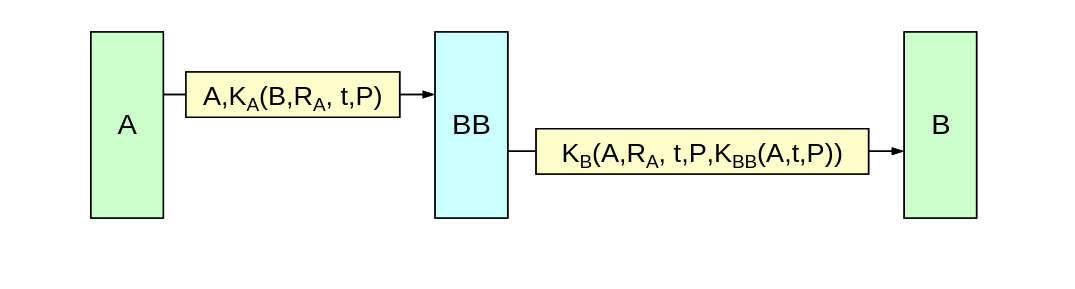
\includegraphics[width=0.8\textwidth]{images/big_brother.png}
        \caption{Big Brother}
    \end{figure}
    \item \textbf{Firma digital con clave asimétrica:} Se utilizan dos claves, una pública y otra privada. El emisor firma el mensaje con su clave privada y el receptor verifica la firma con la clave pública del emisor.
\end{itemize}

\subsubsection{El concepto de \textit{Big Brother} en la firma digital}

El concepto de \textit{Big Brother} en la firma digital se refiere a un escenario donde una autoridad central o entidad de confianza supervisa, regula y controla el proceso de autenticación y verificación de firmas digitales. Esta idea se asemeja a un sistema donde todos los actores confían en una única entidad para garantizar la seguridad e integridad de las operaciones. A continuación, se describen los pasos fundamentales en este esquema:

\begin{enumerate}
    \item \textbf{Generación de claves:} Cada usuario genera un par de claves criptográficas (una clave pública y una clave privada). La clave pública es registrada y almacenada por la autoridad central (el \textit{Big Brother}).
    \item \textbf{Emisión de certificados:} La autoridad central emite certificados digitales para asociar cada clave pública con la identidad del usuario. Estos certificados son firmados digitalmente por la autoridad, lo que les otorga validez y confiabilidad.
    \item \textbf{Creación de la firma:} Para firmar un documento, el usuario utiliza su clave privada. Este proceso produce una firma digital única, basada en el contenido del documento y en la clave privada del usuario.
    \item \textbf{Verificación de la firma:} La parte receptora utiliza la clave pública del usuario para verificar la autenticidad de la firma digital. La validez de la clave pública y su asociación con la identidad del firmante se confirman consultando el certificado digital emitido por la autoridad central.
    \item \textbf{Control y supervisión:} La autoridad central actúa como un garante del sistema, asegurando que las claves públicas y los certificados estén actualizados y evitando posibles fraudes o duplicaciones.
\end{enumerate}

Este modelo tiene la ventaja de centralizar la confianza, simplificando el proceso para los usuarios finales. Sin embargo, también presenta desafíos significativos, como la dependencia total de la autoridad central, que puede convertirse en un único punto de falla en el sistema.
\newpage




El proceso de firma digital con clave asimétrica se puede describir mediante un doble cifrado:

\begin{figure}[H]
    \centering
    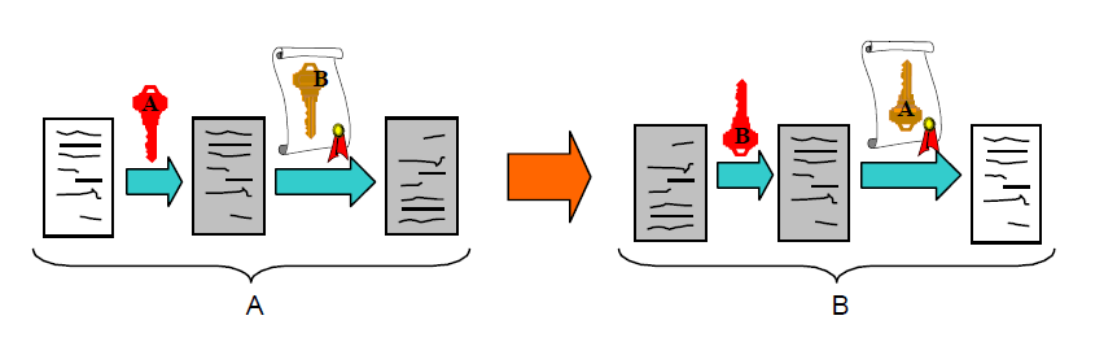
\includegraphics[width=0.8\textwidth]{images/cifrado_ej.png}
    \caption{Proceso de firma digital con clave asimétrica.}
\end{figure}

\begin{enumerate}
    \item Primero, para proporcionar privacidad, el mensaje \( T \) es cifrado con la clave pública \( K_{\text{pubB}} \) del receptor.
    \item Luego, para autenticación, se cifra previamente con la clave privada \( K_{\text{priA}} \) del emisor.
    \item El mensaje firmado se envía como \( K_{\text{pubB}}( K_{\text{priA}}( T ) ) \).
    \item El receptor, al recibir el mensaje, lo descifra primero con su clave privada \( K_{\text{priB}} \), luego con la clave pública del emisor \( K_{\text{pubA}} \), y finalmente obtiene el mensaje original \( T \).
\end{enumerate}



\subsubsection{Debilidad y Garantía de No Repudio}

Una de las debilidades del sistema es que para garantizar el \textit{no repudio}, se necesita asegurar la asociación indisoluble entre la ''identidad A'' y su ''clave pública \( K_{\text{pubA}} \)''. Esto es necesario para garantizar que el emisor no pueda negar su identidad al haber firmado el mensaje.

Para resolver este problema, se utiliza un \textit{certificado digital}, que garantiza la asociación entre una identidad y una clave pública.

\subsubsection{Certificados Digitales}

Un \textit{certificado digital} es un documento que asocia de manera fidedigna una identidad a una clave pública. El proceso de obtención y verificación de un certificado digital incluye los siguientes pasos:

\begin{itemize}
    \item El usuario genera su par de claves pública y privada.
    \item El usuario envía una solicitud a una \textit{Autoridad de Certificación} (AC), firmada digitalmente, indicando su identidad y su clave pública.
    \item La AC verifica la firma y, si todo es correcto, emite un certificado digital que contiene:
    \begin{itemize}
        \item La identidad de la AC.
        \item La identidad del usuario.
        \item La clave pública del usuario.
        \item Otros datos, como el período de validez del certificado.
    \end{itemize}
    \item El certificado es firmado digitalmente por la AC, utilizando su clave privada, para evitar su falsificación.
\end{itemize}

\subsubsection{Formato de los Certificados}

El formato más común para los certificados digitales es el estándar \textit{X.509}. Este formato asegura que los certificados sean compatibles entre diferentes sistemas y aplicaciones.

\subsubsection{Autoridades de Certificación (AC) Reconocidas}

Algunas de las Autoridades de Certificación más reconocidas incluyen:

\begin{itemize}
    \item ACE (www.ace.es)
    \item VeriSign (www.verisign.com)
    \item CAMERFIRMA (www.camerfirma.es)
    \item CERES (www.cert.fnmt.es)
\end{itemize}

\subsubsection{Campos de un certificado \textit{X.509}}

\begin{figure}[H]
    \centering
    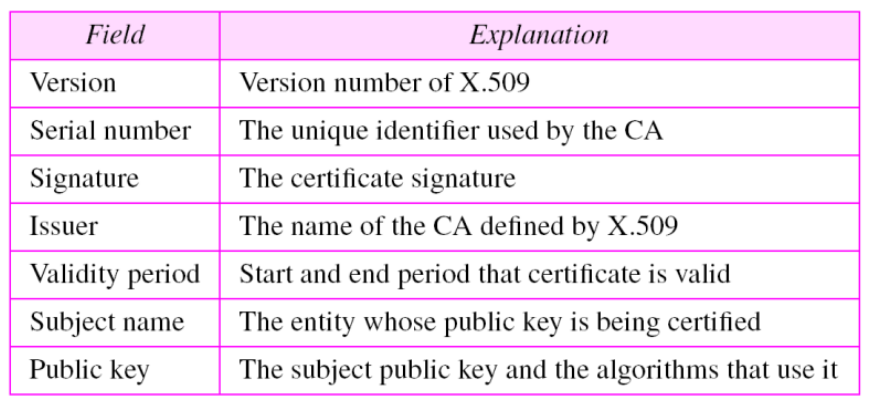
\includegraphics[width=0.8\textwidth]{images/campos_certificado.png}
    \caption{Campos de un certificado X.509.}
\end{figure}

\footnotetext{Para más información de un certificado X.509 accede a la diapositiva 28 del tema 4.}

\subsection{Relación entre los Mecanismos de Seguridad y los Servicios/Aspectos de Seguridad}

Existen varios mecanismos de seguridad que ayudan a garantizar los diferentes aspectos de la seguridad en los sistemas informáticos. A continuación, se describe la relación entre los mecanismos de seguridad y los servicios de seguridad más importantes:

\subsubsection{Confidencialidad}

La \textit{confidencialidad} se refiere a garantizar que solo las partes autorizadas puedan acceder a la información. Se consigue mediante el uso de cifrado, que puede ser de dos tipos:

\begin{itemize}
    \item \textbf{Cifrado simétrico:} Utiliza una única clave secreta compartida entre el emisor y el receptor para cifrar y descifrar el mensaje.
    \item \textbf{Cifrado asimétrico:} Utiliza un par de claves, una pública y una privada, donde el emisor cifra el mensaje con la clave pública del receptor y el receptor descifra con su clave privada.
\end{itemize}

Ambos métodos permiten garantizar que la información permanezca confidencial durante su transmisión.

\subsubsection{Autenticación}

La \textit{autenticación} asegura que el receptor pueda verificar la identidad del emisor. Se consigue mediante varios mecanismos, como:

\begin{itemize}
    \item \textbf{Reto-respuesta:} El receptor envía un reto (por ejemplo, una pregunta o desafío) al emisor, quien debe responder correctamente para probar su identidad.
    \item \textbf{Firma digital (Big Brother, doble cifrado):} La firma digital asegura que un mensaje provenga de una fuente específica. En el doble cifrado, el mensaje es cifrado primero con la clave pública del receptor para garantizar la privacidad y luego con la clave privada del emisor para garantizar la autenticidad.
\end{itemize}

\subsubsection{No Repudio}

El \textit{no repudio} significa que el emisor no puede negar haber enviado un mensaje una vez que ha sido firmado. Este aspecto de la seguridad se logra mediante:

\begin{itemize}
    \item \textbf{Firma digital (Big Brother, doble cifrado):} Al firmar digitalmente un mensaje con la clave privada del emisor, se asegura que solo él pudo haberlo firmado, lo que impide que pueda negar su participación en la transmisión del mensaje.
\end{itemize}

\subsubsection{Integridad}

La \textit{integridad} garantiza que el mensaje no haya sido alterado durante la transmisión. Se consigue mediante:

\begin{itemize}
    \item \textbf{Compendios o resúmenes:} Se genera un valor hash del mensaje utilizando funciones hash. Este valor se adjunta al mensaje como un resumen, y cualquier alteración del mensaje cambiará el resumen, lo que permite detectar la manipulación.
\end{itemize}

\subsubsection{Disponibilidad}

La \textit{disponibilidad} se refiere a asegurar que los servicios y recursos estén disponibles para los usuarios autorizados cuando los necesiten. Sin embargo, los mecanismos de seguridad mencionados anteriormente no proporcionan disponibilidad por sí solos. Para garantizar la disponibilidad, se requieren:

\begin{itemize}
    \item \textbf{Sistemas antiataque:} Para proteger contra ataques de denegación de servicio (DoS) y otros que puedan afectar la disponibilidad.
    \item \textbf{Redundancia:} La redundancia en las líneas de acceso y en los servidores garantiza que, en caso de fallo de un sistema, otro pueda tomar su lugar y continuar brindando los servicios.
\end{itemize}

\section{Protocolos Seguros}

\subsection{Seguridad}

\subsection*{Seguridad Perimetral}

La \textit{seguridad perimetral} se refiere a la protección de las redes de comunicaciones de una organización contra accesos no autorizados o ataques desde el exterior. Para ello, se utilizan diversos mecanismos de seguridad, entre los que destacan:

\begin{itemize}
    \item \textbf{Firewalls:} Son dispositivos o software que filtran el tráfico de red entre diferentes zonas, como la red interna y la externa, permitiendo o bloqueando conexiones según un conjunto de reglas predefinidas.
    \item \textbf{Sistemas de detección de intrusiones (IDS):} Son sistemas que monitorean el tráfico de red en busca de patrones o comportamientos sospechosos que puedan indicar un intento de intrusión.
    \item \textbf{Sistemas de respuesta a intrusiones (IRS):} Estos sistemas no solo detectan intrusiones, sino que también responden a ellas de manera automática, por ejemplo, bloqueando el acceso a ciertos recursos o alertando a los administradores.
\end{itemize}

\subsection*{Seguridad Criptográfica en Protocolos}

La seguridad en los protocolos de comunicación se puede aplicar en diferentes capas del modelo OSI, cada una con sus propias soluciones de seguridad:

\subsubsection*{Capa de Aplicación}

En la capa de aplicación se implementan mecanismos de seguridad para proteger las comunicaciones a nivel de la aplicación. Algunos ejemplos son:

\begin{itemize}
    \item \textbf{Pretty Good Privacy (PGP):} Es un protocolo de cifrado utilizado para la protección de correos electrónicos. PGP ofrece confidencialidad mediante cifrado, autenticación mediante firma digital y garantiza la integridad del mensaje mediante un hash.
    \item \textbf{Secure Shell (SSH):} Protocolo utilizado para acceder de manera segura a máquinas remotas, proporcionando cifrado de los datos, autenticación del servidor y del cliente, y confidencialidad en la comunicación.
\end{itemize}

\subsubsection*{Capa de Sesión (Entre Aplicación y Transporte)}

En esta capa, la seguridad se implementa mediante protocolos que proporcionan seguridad en la comunicación entre la capa de aplicación y la capa de transporte:

\begin{itemize}
    \item \textbf{Transport Layer Security (TLS):} Es un protocolo criptográfico que proporciona seguridad en las comunicaciones a través de la red. TLS, que anteriormente era conocido como SSL (Secure Sockets Layer), se utiliza en protocolos como HTTPS, IMAPS, SSL-POP y VPN. TLS ofrece:
    \begin{itemize}
        \item \textbf{Confidencialidad:} Mediante una clave secreta negociada entre el cliente y el servidor.
        \item \textbf{Autenticación:} El servidor se autentica por defecto mediante su clave pública (KPUBLICA).
        \item \textbf{Integridad:} Utilizando el algoritmo HMAC (Hash-based Message Authentication Code) para asegurar que los datos no han sido modificados durante la transmisión.
    \end{itemize}
    \item \textbf{TLS Handshake:} El proceso de \textit{Handshake} se utiliza para negociar los parámetros de seguridad antes de que los datos sean transmitidos. Esto incluye la negociación de la clave secreta y la autenticación del servidor.
    \item \textbf{TLS Record Protocol:} Después del \textit{Handshake}, el protocolo de registro se encarga de cifrar y autenticar los datos transmitidos.
\end{itemize}

\subsubsection*{Capa de Red}

En la capa de red se implementan mecanismos de seguridad para proteger el tráfico de red en su totalidad. Un ejemplo de ello es:

\begin{itemize}
    \item \textbf{IPSec (VPN):} IPSec es un conjunto de protocolos que proporcionan seguridad a nivel de red, protegiendo los datos a través de la encriptación y autenticación. Se utiliza principalmente en redes privadas virtuales (VPN), proporcionando confidencialidad, autenticación de los paquetes de datos y protección contra ataques de modificación.
\end{itemize}











\subsection{Pretty Good Privacy (PGP) -- correo electrónico seguro}

\begin{figure}[H]
    \centering
    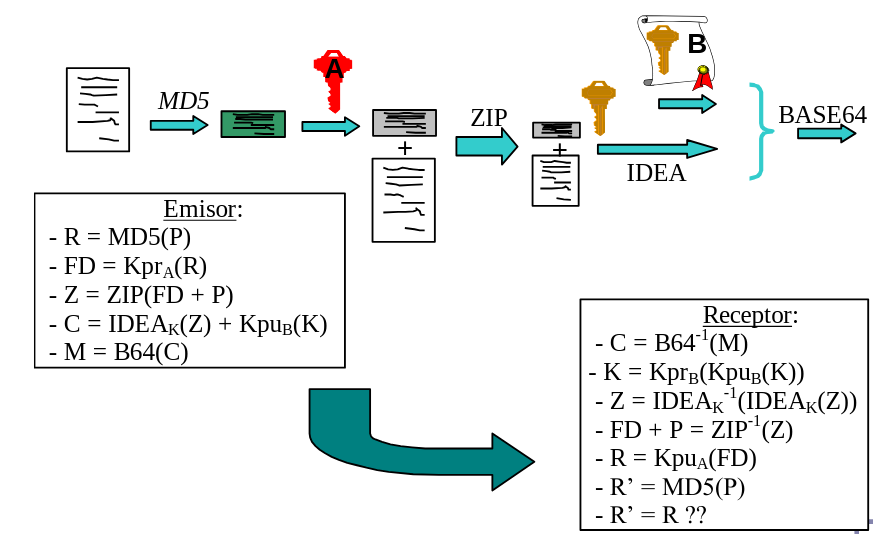
\includegraphics[width=0.8\textwidth]{images/pgp.png}
    \caption{Pretty Good Privacy (PGP).}
\end{figure}

\subsubsection*{Proceso de Cifrado y Descifrado en PGP}

PGP (Pretty Good Privacy) es un método de cifrado para la comunicación segura por correo electrónico. A continuación se detalla el proceso de cifrado y descifrado utilizado en PGP.

\subsubsection*{Cifrado por el Emisor}
\begin{enumerate}
    \item \textbf{Generación de Resumen}: Se genera un resumen del mensaje original \(P\) usando el algoritmo MD5:
    \begin{equation}
        R = \text{MD5}(P)
    \end{equation}
    \item \textbf{Firma Digital}: Se cifra el resumen utilizando la clave privada del emisor \(K_{\text{prA}}\):
    \begin{equation}
        FD = K_{\text{prA}}(R)
    \end{equation}
    \item \textbf{Compresión}: Se comprimen la firma digital y el mensaje original:
    \begin{equation}
        Z = \text{ZIP}(FD + P)
    \end{equation}
    \item \textbf{Cifrado del Mensaje}: Se cifra el mensaje comprimido usando el algoritmo IDEA y una clave de sesión \(K\). Además, se cifra la clave de sesión usando la clave pública del receptor \(K_{\text{pubB}}\):
    \begin{equation}
        C = \text{IDEA}_K(Z) + K_{\text{pubB}}(K)
    \end{equation}
    \item \textbf{Codificación Base64}: El mensaje cifrado se codifica en formato Base64 para su transmisión:
    \begin{equation}
        M = \text{B64}(C)
    \end{equation}
\end{enumerate}

\subsubsection*{Descifrado por el Receptor}
\begin{enumerate}
    \item \textbf{Decodificación Base64}: El receptor decodifica el mensaje del formato Base64:
    \begin{equation}
        C = \text{B64}^{-1}(M)
    \end{equation}
    \item \textbf{Descifrado de la Clave de Sesión}: El receptor descifra la clave de sesión usando su clave privada \(K_{\text{prB}}\):
    \begin{equation}
        K = K_{\text{prB}}(K_{\text{pubB}}(K))
    \end{equation}
    \item \textbf{Descifrado del Mensaje}: Se descifra el mensaje comprimido usando la clave de sesión:
    \begin{equation}
        Z = \text{IDEA}_K^{-1}(C)
    \end{equation}
    \item \textbf{Descompresión}: Se descomprime el mensaje para obtener la firma digital y el mensaje original:
    \begin{equation}
        FD + P = \text{ZIP}^{-1}(Z)
    \end{equation}
    \item \textbf{Verificación de la Firma}: Se descifra la firma digital usando la clave pública del emisor \(K_{\text{puA}}\):
    \begin{equation}
        R = K_{\text{puA}}(FD)
    \end{equation}
    \item \textbf{Verificación del Resumen}: Se genera un resumen del mensaje recibido y se compara con el resumen cifrado recibido:
    \begin{equation}
        R' = \text{MD5}(P)
    \end{equation}
    \begin{equation}
        R' \stackrel{?}{=} R
    \end{equation}
\end{enumerate}





\subsection{Transport Layer Security (TLS) / Secure Sockets Layer (SSL)}

El protocolo \textit{Transport Layer Security (TLS)} (anteriormente conocido como \textit{Secure Sockets Layer (SSL)}) proporciona seguridad en las comunicaciones de red a través de la confidencialidad, autenticación e integridad. Se utiliza ampliamente en protocolos como \textbf{HTTPS}, \textbf{IMAPS}, \textbf{SSL-POP} y \textbf{VPN}.

\subsubsection{SSL Record Protocol}

El \textit{SSL Record Protocol}\footnote{Para ver imágenes sobre este apartado revisa las diapositivas 33 y 34 del tema 4} encapsula los datos de otros protocolos y ofrece un canal seguro que garantiza:

\begin{itemize}
    \item \textbf{Privacidad:} A través de la encriptación de los datos.
    \item \textbf{Autenticación:} Garantizando que el servidor es quien dice ser.
    \item \textbf{Integridad:} Usando técnicas de hash para asegurar que los datos no sean modificados durante la transmisión.
\end{itemize}

Este protocolo se encarga de fragmentar, comprimir y cifrar los datos antes de su transmisión a través de la red.

\subsubsection{SSL Handshake Protocol}

El \textit{SSL Handshake Protocol} es el proceso mediante el cual el cliente y el servidor negocian los parámetros de seguridad antes de la transmisión de datos. Este protocolo realiza las siguientes funciones clave:

\begin{itemize}
    \item \textbf{Negociación del algoritmo de cifrado:} El cliente y el servidor acuerdan qué algoritmo de cifrado utilizar para proteger la comunicación.
    \item \textbf{Negociación de la función hash:} Se selecciona la función hash que se utilizará para garantizar la integridad de los datos.
    \item \textbf{Autenticación del servidor:} El servidor se autentica utilizando un certificado X.509, lo que permite al cliente verificar su identidad.
\end{itemize}

\subsubsection{Generación de Claves de Sesión}

Durante el proceso de \textit{handshake}, se generan las claves de sesión necesarias para proteger la comunicación. Estas claves se generan de la siguiente manera:

\begin{itemize}
    \item \textbf{Claves aleatorias cifradas con la clave pública del servidor (KPUB\_SERVER):} El cliente genera claves de sesión aleatorias que son cifradas con la clave pública del servidor para asegurar su confidencialidad.
    \item \textbf{Diffie-Hellman:} Alternativamente, se puede utilizar el protocolo Diffie-Hellman para intercambiar de manera segura una clave compartida sin necesidad de transmitirla directamente.
\end{itemize}

\subsubsection{SSL Assert Protocol}

El \textit{SSL Assert Protocol} es utilizado para informar sobre cualquier error o anomalía detectada durante la sesión, asegurando que las partes involucradas puedan reaccionar ante posibles problemas de seguridad.

\subsubsection{Change Cipher Spec Protocol}

El \textit{Change Cipher Spec Protocol} notifica cualquier cambio en la configuración del cifrado durante una sesión SSL/TLS. Este protocolo se utiliza para asegurarse de que tanto el cliente como el servidor estén de acuerdo en los cambios realizados en los parámetros de cifrado, como el algoritmo o las claves de sesión.

\subsubsection{Protocolos Utilizados con TLS/SSL}

TLS/SSL es utilizado en una variedad de protocolos para asegurar la comunicación. Algunos ejemplos incluyen:

\begin{itemize}
    \item \textbf{HTTPS:} Protocolo de transferencia de hipertexto seguro utilizado para comunicaciones seguras en la web.
    \item \textbf{IMAPS:} Protocolo de acceso a mensajes de internet seguro, utilizado para acceder a correos electrónicos de manera segura.
    \item \textbf{SSL-POP:} Protocolo de oficina de correos seguro, usado para acceder a correos electrónicos en servidores POP.
    \item \textbf{VPN:} Redes privadas virtuales que utilizan TLS/SSL para crear túneles seguros entre redes.
\end{itemize}




\subsection{IPSec}

El objetivo principal de \textit{IPSec}\footnote{Para ver imágenes sobre este apartado revisa las diapositivas 36 del tema 4} es garantizar la \textit{autenticación}, \textit{integridad} y, opcionalmente, la \textit{privacidad} a nivel de la capa IP. Este conjunto de protocolos se utiliza para asegurar las comunicaciones a través de redes IP, proporcionando confidencialidad e integridad en los datos.

\subsubsection{Procedimientos de IPSec}

IPSec se compone de tres procedimientos clave:

\begin{enumerate}
    \item \textbf{Establecimiento de una Asociación de Seguridad:} 
    \begin{itemize}
        \item Utiliza el protocolo \textit{IKE (Internet Key Exchange)} especificado en la \textbf{RFC 2409}.
        \item El objetivo es establecer una clave secreta compartida entre los participantes, usando el protocolo \textit{Diffie-Hellman}.
        \item Incluye una autenticación previa de los participantes, mediante certificados, para evitar el ataque de \textit{hombre en el medio}.
        \item La asociación de seguridad es \textit{simplex}, lo que significa que tiene un único sentido, es decir, se establece para un único flujo de datos.
        \item La asociación se identifica mediante la combinación de la IP de origen y un \textit{Security Parameter Index (SPI)} de 32 bits.
        \item Una de las limitaciones de este procedimiento es que vulnera el carácter \textit{no orientado a conexión} de la capa IP.
    \end{itemize}

    \item \textbf{Garantizar la Autenticación e Integridad de los Datos:} 
    \begin{itemize}
        \item Se utiliza el protocolo de \textit{Cabeceras de Autenticación} especificado en la \textbf{RFC 2401}.
        \item Este protocolo asegura que los datos transmitidos no hayan sido alterados y autentica a los participantes en la comunicación.
    \end{itemize}

    \item \textbf{(Opcional) Garantizar la Autenticación, Integridad y Privacidad de los Datos:} 
    \begin{itemize}
        \item Se utiliza el protocolo de \textit{Encapsulado de Seguridad de la Carga} especificado en la \textbf{RFC 2411}.
        \item Este protocolo garantiza tanto la integridad como la confidencialidad de los datos, cifrando la carga útil de los paquetes.
    \end{itemize}
\end{enumerate}

\subsubsection{Modos de Operación de IPSec}

IPSec puede operar en dos modos diferentes, según el alcance de la protección que se desea ofrecer:

\begin{itemize}
    \item \textbf{Modo Transporte:} 
    \begin{itemize}
        \item En este modo, la asociación de seguridad se establece entre el host de origen y el host de destino de forma directa, asegurando los datos a nivel de la comunicación entre estos dos puntos finales.
    \end{itemize}
    \item \textbf{Modo Túnel:} 
    \begin{itemize}
        \item En el modo túnel, la asociación de seguridad se establece entre dos routers intermediarios, de manera que todo el tráfico entre estos routers se encuentra protegido, creando un \textit{túnel} seguro para los datos que se transmiten a través de la red.
    \end{itemize}
\end{itemize}





\end{document}